\documentclass[a4paper, 11pt]{article}
\usepackage[text={170mm, 240mm}, left=20mm, top=30mm]{geometry}
\usepackage[utf8]{inputenc}
\usepackage[czech]{babel}
\usepackage{times}
\usepackage[dvipsnames]{xcolor}
\usepackage{graphicx}
\usepackage{hyperref}

\begin{document}
\begin{titlepage}
\vspace*{\fill}
\noindent {\fontsize{65}{50} \color{ForestGreen} \textsc{Calc-chan}} {\Large \textsc{by Paks}}\\[0.3em]
{\fontsize{40}{40}\textsc{Uživatelský manuál}}
\vspace*{\fill}
\end{titlepage}
	
\tableofcontents

\newpage

\section{Úvod}
Calc-chan je jednoduchá aplikace pro vyhodnocování jednoduchých matematických výrazů. Mezi matematické funkce, které Calc-chan nabízí patří sčítání, odčítání, násobení, dělení, mocnina, obecná odmocnina, faktoriál a přirozený logaritmus.

\section{Prerekvizity}
Aplikace byla vyvinuta v programovacím jazyce Python3 a pro grafické rozhraní využívá také knihovnu Python3 tkinter. Instalátor však tento problém řeší za uživatele a prerekvizity nainstaluje sám.

\section{Instalace a spuštění}
K nainstalování aplikace Calc-chan je potřeba stáhnout instalátor \texttt{\textbf{cchan.deb}}.
\subsection{Instalace z terminálu}
\noindent Po stažení instalátoru a po přesunu do adresáře ve kterém se nachází je možné instalátor spustit následujícím příkazem:\\
\texttt{\textbf{sudo apt install ./cchan.deb}}\\
\begin{center}
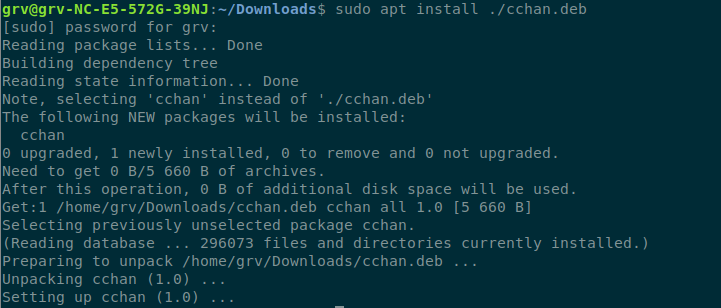
\includegraphics[scale=0.65]{installterminal.png}\\
\end{center}
\newpage
\subsection{Instalace z průzkumníka}
\noindent Alternativně je možné se do stejného adresáře přesunout skrze průzkumníka a instalátor spustit dvojím kliknutím na instalátor. Zobrazí se okno s informacemi o aplikaci a možností instalace.\\
\begin{center}
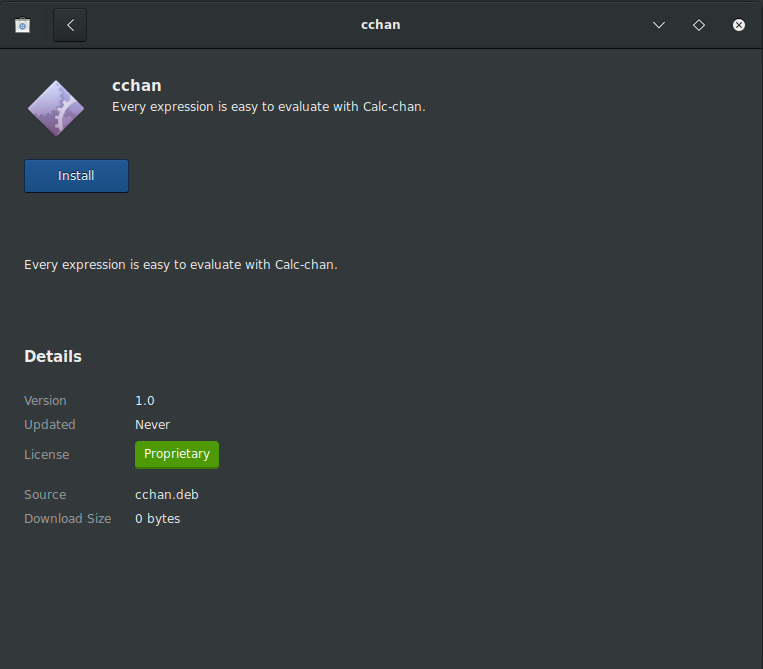
\includegraphics[scale=0.60]{installmanager.png}\\
\end{center}
\newpage
\noindent Po instalaci je možné aplikaci Calc-chan spustit z libovolného adresáře příkazem \texttt{\textbf{cchan}}.\\
\begin{center}
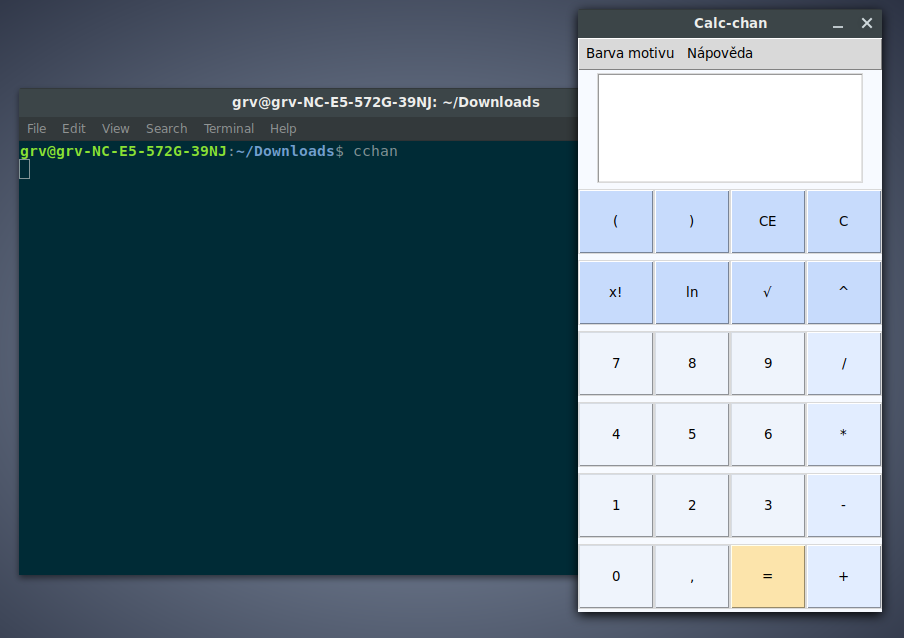
\includegraphics[scale=0.5]{cchanrun}
\end{center}

\newpage
\section{Používání aplikace}
Aplikaci lze ovládat pomocí tlačítek pod displejem, kromě toho je také možné zadávat výrazy k vyhodnocení pomocí klávesnice do displeje přímo, stačí myší kliknout kamkoliv do prostoru displeje.
\subsection{Menu}
\begin{itemize}
\item Tlačítko \texttt{Barva motivu}\\Slouží k výběru motivu, více v následující kapitole.
\item Tlačítko \texttt{Nápověda}\\Zobrazí nápovědu s vysvětlivkami ke speciálním tlačítkům aplikace.
\end{itemize}
\subsection{Tlačítka operandů}
\begin{itemize}
\item Tlačítka \texttt{0 - 9}\\K dispozici jsou tlačítka číslic 0 až 9, po stisknutí libovolného z nich se přidá do výrazu na displeji odpovídající číslice.
\item Tlačítko \texttt{.}\\Slouží k zápisu desetinného čísla. Možný validní výraz: 5.5
\end{itemize}
K dispozici jsou tlačítka číslic 0 až 9, po stisknutí libovolného z nich se na displeji zobrazí odpovídající císlice. Kromě tlačítek číslic je k dispocizi také tlačítku \texttt{.}, které značí desetinnou tečku.
\subsection{Základní aritmetické operace}
\begin{itemize}
\item Tlačítko \texttt{+}\\Značí matematickou operaci součet. Možný validní zápis: 5+5
\item Tlačítko \texttt{-}\\Značí matematickou operaci rozdíl. Možný validní zápis: 5-5
\item Tlačítko \texttt{*}\\Značí matematickou operaci součin. Možný validní zápis: 5*5
\item Tlačítko \texttt{/}\\Značí matematickou operaci podíl. Možný validní zápis: 5/5
\end{itemize}
\subsection{Složitější matematické operace}
\begin{itemize}
\item Tlačítko \texttt{x!}\\Značí matematickou operaci faktoriál. Možný validní zápis: 5!
\item Tlačítko \texttt{ln}\\Značí matematickou operaci přirozený logaritmus. Možný validní zápis: ln(5)
\item Tlačítko \texttt{\^}\\Značí matematickou operaci mocnina. Výraz mocniny se skládá ze základu a exponentu. Možný validní zápis: 5\string^2
\item Tlačítko \texttt{$\sqrt{}$}\\Značí matematickou operaci odmocnina. Výraz odmocniny se skládá ze základu a stupně odmocniny. Číslo před odmocninou je stupeň odmocniny, aplikace považuje $\sqrt{}$ za druhou odmocninu. Možný validní zápis: $\sqrt{25}$
\end{itemize}
\subsection{Speciální tlačítka}
\begin{itemize}
\item Tlačítko \texttt{(}\\Značí levou závorku. Závorky lze použít ke specifikování priority vyhodnocení výrazů. Lze je také použít k tvorbě složitějších výrazů k vyhodnocení. Kromě toho je aplikace používá k odlišení záporného čísla od kladného: -5\string^2 $=$ -25 -- zde se nejprve vyhodnotí výraz 5\string^2 a poté se přidá záporné znaménko. Zatímco výraz (-5)\string^2 aplikace interpretuje jako druhou mocninu čísla -5, tedy -5\string^2 = 25. Možné validní zápisy: (5+5), ln((6+5)\string^(6+9))
\item Tlačítko \texttt{)}\\Značí pravou závorku. Má stejné použití jako levá závorka, kromě toho se také používá k uzavření výrazu obsahujícím přirozený logaritmus, jelikož vyžadovaný zápis je: ln(5)
\item Tlačítko \texttt{=}\\Značí rovnítko. Stisknutím tohohle tlačítka se provede vyhodnocení výrazu zadaného na displeji. Možné výpisy na displeji po vyhodnocení výrazu:
\begin{itemize}
\item Číselný výsledek\\Zadaný výraz je validní a aplikace jej byla schopna vyhodnotit.
\item Syntax error\\Zadaný výraz není validní, aplikace jej nebyla schopna vyhodnotit. Stisknutím libovolného tlačítka je nápis odstraněn a začíná nový zápis výrazu. Příklady syntaktický špatných výrazů: 5++5, ln(\string^), 5$\sqrt{}$, vyjímkou je zde dvojí použítí znaménka mínus, takovou situaci aplikace vyhodnocuje jako změnu znaménka.
\item Value error\\Zadaný výraz obsahuje sémantickou konstrukci, jejíž vyhodnocování buď není možné, nebo ji aplikace nepodporuje. Příklad
\item Zero division\\Zadaný výraz obsahuje dělení nulou, může se jednat o přímé dělení nulou 5/0, nebo o nepřímé dělení nulou po vyhodnocení dílčího výrazu 5/(3-3).
\end{itemize}
\item Tlačítko \texttt{CE}\\Stisknutí tlačítka CE má za následek umazání posledního znaku ve výrazu, nebo umazání znaku před kurzorem v poli displeje pokud je aktivní.
\item Tlačítko \texttt{C}\\Stisknutí tlačítka C má za následek smazání veškerého obsahu displeje a vyresetování do původního stavu kdy je aplikace připravena na zadání výrazu. 
\end{itemize}
\newpage
Ukázka výpočtu:\vspace{20pt}\\
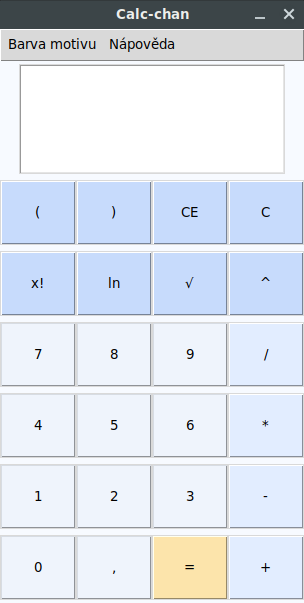
\includegraphics[scale=0.5]{calc1.png}
\hspace{10pt}
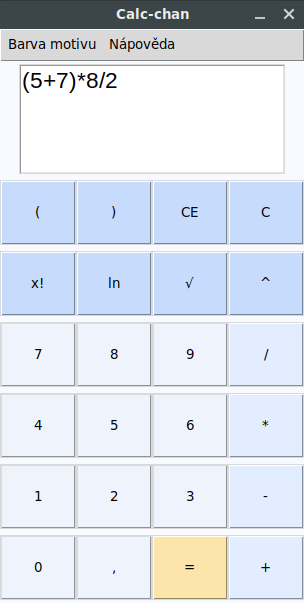
\includegraphics[scale=0.5]{calc2.png}
\hspace{10pt}
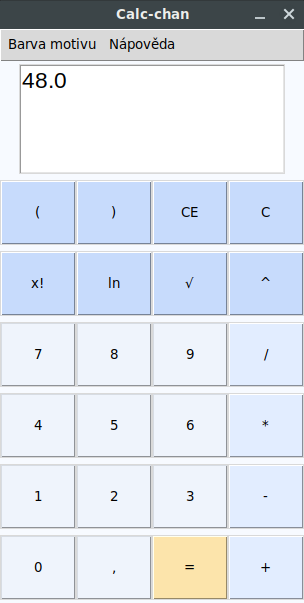
\includegraphics[scale=0.5]{calc3.png}
\newpage
\section{Barevné motivy}
Calc-chan nabízí uživateli výběr ze dvou barevných motivů -- světlého a tmavého. Motiv se dá změnit v kontextovém menu po kliknutí na tlačítko \texttt{Barva motivu}.\\
\begin{center}
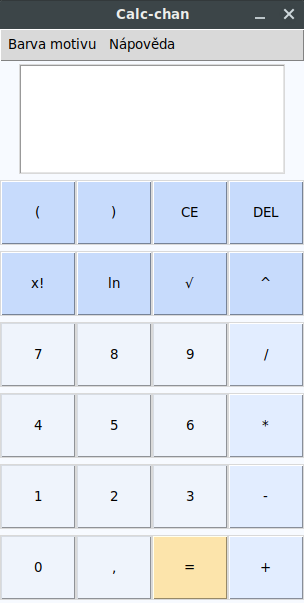
\includegraphics[scale=0.5]{screenshot.png}
\hspace{50pt}
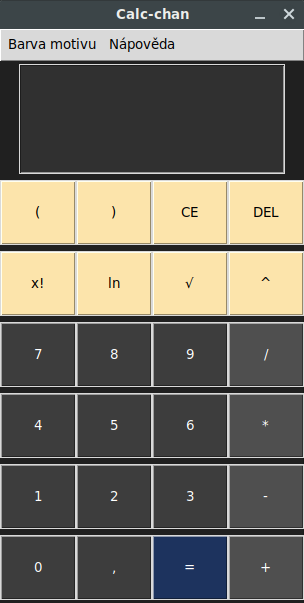
\includegraphics[scale=0.5]{screenshot2.png}
\end{center}



\end{document}